\documentclass[a4paper, 12pt, oneside, openany]{book}

%\renewcommand{\familydefault}{\sfdefault}
\usepackage{fontspec}
\usepackage[svgnames]{xcolor}
\usepackage[ngerman]{babel}
\usepackage{framed}
%\usepackage[utf8]{inputenc}
%\usepackage[T1]{fontenc}
\babelprovide[import=ja, script=Kana]{japanese}

\defaultfontfeatures{Scale=MatchUppercase, Ligatures=TeX}

\babelfont{rm}[
   Ligatures = {Discretionary, TeX},
   UprightFont = *-regular ,
   BoldFont = *-bold ,
   ItalicFont = *-regularit ,
   BoldItalicFont = *-boldit ,
   Extension = .ttf ]{cmss}

\usepackage{csquotes}
\MakeOuterQuote{"}

\usepackage{tikz}
\usepackage{booktabs}
\usepackage{lipsum}
\usepackage{graphicx}
\usepackage{amsmath, amsfonts, amssymb}
\usepackage[skins]{tcolorbox}
\usepackage{makecell}

\setlength\parindent{0pt}

\usepackage{etoolbox}
\patchcmd{\chapter}{\if@openright\cleardoublepage\else\clearpage\fi}{}{}{}

\usepackage{titlesec}
\titleformat{\chapter}[display]
{\normalfont\huge\bfseries}{}{20pt}{\Huge}
\titlespacing*{\chapter}{0pt}{-50pt}{40pt}

\renewcommand{\arraystretch}{1.2}

\usepackage{geometry}
\geometry{
	left=3cm,
	right=3cm,
	footskip=0.5cm,
	bottom=3.9cm
}
\renewcommand*\baselinestretch{1.2}\selectfont

\newcommand{\definition}[2]{
  	\refstepcounter{subsection}%
  	\addcontentsline{toc}{subsection}{\protect\numberline{\thesubsection}#1}%
  	\subsectionmark{#1}
	\hfil
	\begin{tcolorbox}
	[colback=white, colframe=red!75!black, fonttitle=\bfseries\large, title=#1]
	#2
	\end{tcolorbox}
	\hfil
}

\newcommand{\example}[1]{
	\begin{minipage}{\linewidth}
	\textbf{\large Beispiel}\\[0.7em]
	\setlength{\parindent}{0.5cm}
	\indent
	#1
	\noindent
	\setlength{\parindent}{0pt}
	\end{minipage}
	\\
}


\begin{document}
	\begin{titlepage}
	\raggedleft

	\vspace*{\baselineskip}

	{\Large Semesterprojekt "Dialoge mit Computern"\\an der Humboldt-Universität Berlin}

	\vspace*{0.167\textheight}

	\textbf{\LARGE Leanoard Fiedrowicz \& Marc Zierle}\\[\baselineskip]

	{\textcolor{Red}{\textbf{\Huge Der JANUS ChatBot}}}\\[\baselineskip]

	{\Large \textit{Termine automatisch plannen lassen}}

	\vfill

	%{\large Lorem ipsum}

	\vspace*{3\baselineskip}
\end{titlepage}


	\tableofcontents

	\chapter{Einführung}
\section{Motivation und Idee}

Am Samstag zu 14 Uhr zum Zahnarzt. Anschließend ein treffen mit der Familie. Und eingekauft werden muss ja auch noch irgendwann. In der heutigen Welt kann es zunehmend schwieriger werden, alle Termine im Auge zu behalten und dabei eine möglichst effiziente Zeitplanung zu betreiben.\\

Genau dort setzt unser JANUS-Chatbot an. Nutzer sollen in der Lage sein, ihre Termine und Ereignisse dem Chatbot anzuvertrauen und nebenbei plant JANUS vollautomatisiert jene Termine, für die lediglich bekannt ist, wie viel Zeit sie einnehmen werden, jedoch noch kein genaues Datum feststeht. Dabei soll eine möglichst optimale "Route" von Terminen in Bezug zur Fahrzeit von einem Event zum nächsten berücksichtigt werden. 


\section{Anforderungen}
Im Folgenden eine Übersicht der wesentlichen Anforderung an die Funktionalität unseres Chatbots:

\subsection{Terminplanung}
Für einen zuplanenden Termin werden drei Informationen vom Nutzer benötigt und erfragt:
\begin{itemize}
	\item Location - der Ort, an dem der Termin stattfinden wird
	\item Event Name - ein Name, unter dem der Termin dem Nutzer in einer Übersicht angezeigt wird
	\item Time / Duration - eine exaktes Datum samt Uhrzeit an dem der Termin stattfinden wird; alternativ kann auch eine Dauer angegeben werden
\end{itemize}
Nutzer können zwei Arten von Terminen planen, die wir nachfolgend als \textit{spezifische Events} und \textit{unspezifische Events} unterteilen.\\
Die Location und ein Event Name sind Pflichtangaben für jeden zuplanenden Termin. Im Unterschied zu einem spezifischen Termin, bei dem das Datum und die Start- und Enduhrzeit im Vorhinein feststehen, brauch bei einem unspezifischen Termin lediglich eine Dauer in Stunden oder Minuten angegeben werden.\\

Hat ein Nutzer alle seine zuplanenden Termine angegeben, wird JANUS diese in der Art anordnen, sodass die Reisezeit zwischen ihnen möglichst minimiert wird. Dabei beginnt und endet die Planung eines Tages beim Zuhause des Nutzers, wobei jener oder jene den Zeitraum angeben kann, in dem ihm oder ihr eine Terminplanung passt. Im Konkreten gehen wir dabei greedy vor, um einen optimalen Plan gegen eine zu hohe Berechnungszeit abzuwägen. Dabei erzielen wir zwar keine optimalen Pläne im theoretischen Sinne, aber zufriedenstellende Ergebnisse in kurzer Zeit.

\subsection{Anzeigen von Terminen}
Alle Termine, die von einem Nutzer und JANUS geplant wurden, sollen in einer visuellen Repräsentation angezeigt werden können. Draus soll erkenntlich werden, welche Terminzeiten vom Nutzer festgelegt wurden, und welche vom Chatbot. Außerdem erfährt der Nutzer hierüber, wie viel Zeit für eine Fahrt zwischen Terminen benötigt wird.

\subsection{Entfernen von geplanten Terminen}
Einmal geplante Termine soll der Nutzer wieder aus seinem Plan entfernen können. Hierzu wird dem Chatbot ein Tag mitgeteilt, an dem sich der zuentfernende Termin befindet. Daraufhin erhält er oder sie eine Liste aller an diesem Tag geplanten Terminen, aus denen einer zum Entfernen ausgewählt wird.

\subsection{Small-Talk}
Um eine natürliche Konversation mit JANUS zu fördern, sollte der Chatbot auf Anfragen und Antworten außerhalb seines eigentlichen Aufgabenbereichs angemessen reagieren. Beispielsweise sollte auf die Frage "How are you?" die mögliche Antwort "I'm fine. And you?" folgen. 

	
	\chapter{Installation}

Diese Installationsanweisungen wurden auf Ubuntu-Distributionen getestet\\
Superuser-Rechte sind hier vorausgesetzt\\
\\
\\
\\
Öffnen Sie die Konsole und geben Sie folgenden Befehl ein\\

\begin{framed}
\texttt{\$ sudo apt-get install python3 pip3 curl libpcre3 libpcre3-dev git}
\end{framed}
\hfill\\\\
\begin{tabular}{cl}
	python3 & Programm ist in Python geschrieben\\
	pip3 & Für die Installation der nötigen Module\\
	curl & Zum Installieren von stack \\
	libpcre3 & Zum Installieren von stack \\
	libpcre3-dev & Zum Installieren von stack \\
	git & Zum Runterladen von dem ChatBot und Duckling \\
\end{tabular}
\newpage
\begin{framed}
\texttt{\$ pip3 install rasa tensorflow spacy python-dotenv pillow \textbackslash \\ $\phantom{.}\qquad$ iso8601  icalendar}
\end{framed}
\hfill\\\\
\begin{tabular}{cl}
	rasa & Für Natural-Language-Processing und Rasa Core\\
	tensorflow & Benötigt für Rasa\\
	spacy & Benötigt für Rasa\\
	python-dotenv & Zum Laden von .env Dateien für die API-Keys \\
	pillow & Image-Library zum Erstellen von Bilddateien \\
	icalendar & Zum In-/Exportieren von .ical oder .ics Kalender-Dateien \\
	iso8601 & Zum Parsen von String zu Datetime-Objekten 
\end{tabular}
\\\\\\\\
Benötigt für Spacy
\begin{framed}
	\texttt{\$ python3 -m spacy download en\_core\_web\_md \\
		\$ python3 -m spacy link en\_core\_web\_md en}
\end{framed}
\hfill\\\\
Zum Runterladen von dem ChatBot und Duckling. Duckling wird benutzt um Zeiten aus Text zu extrahieren.
\begin{framed}
	\texttt{\$ git clone https://github.com/MarcZierle/ChatBot \\
		\$ cd ChatBot \\ 
		\$ git clone  https://github.com/facebook/duckling}
\end{framed}
\hfill\\\\
\newpage
Zum Installieren von Duckling. Dafür wird Stack benötigt was auch erst installiert werden muss. \texttt{\$ stack build} kann eine Weile zum Installieren benötigen.\\
\begin{framed}
	\texttt{\$ cd duckling \\
	\$ curl -sSL https://get.haskellstack.org/ | sh \\
	\$ stack init \\
	\$ sudo stack build \\
	\$ cd ..}
\end{framed}
\hfill\\\\


Als nächstes muss d Rasa Modell trainiert werden. Dazu einfach das Shell-Skript \texttt{train\_rasa\_model.sh} ausführen. \\
\begin{framed}
	\texttt{\$ ./trains\_rasa\_model.sh}
\end{framed}
\hfill\\
Der ChatBot Ordner muss noch dem \texttt{PYTHONPATH} hinzugefügt werden mit z.B \\
\begin{framed}
	\texttt{\$ export PYTHONPATH="/home/ChatBot"}
\end{framed}
\hfill\\

Der absolute Pfad des ChatBot Ordners muss auch noch in der \texttt{settings.py} eingetragen werden. \\
\begin{framed}
	6$\qquad$ ...\\
	7$\qquad$\texttt{env\_path = Path('/home/ChatBot') / '.env'}\\
	8$\qquad$ ...
\end{framed}
\hfill\\

Danach muss der Help Server für die Custom Actions für Rasa und für Duckling mit \texttt{run\_help\_servers.sh \&} gestartet werden.\\
 \begin{framed}
 	\texttt{\$ ./run\_help\_servers.sh \&}
 \end{framed}
 \hfill\\
 
Zum Starten des Programms dann die \texttt{main.py} starten.\\
  \begin{framed}
 	\texttt{\$ python3 main.py}
 \end{framed}
 \hfill\\\\
 
Nach dem Beenden der \texttt{main.py} kann der Help Server Prozess mit \texttt{\$ pkill rasa} beendet werden.

	
	\chapter{Dialogmodell}

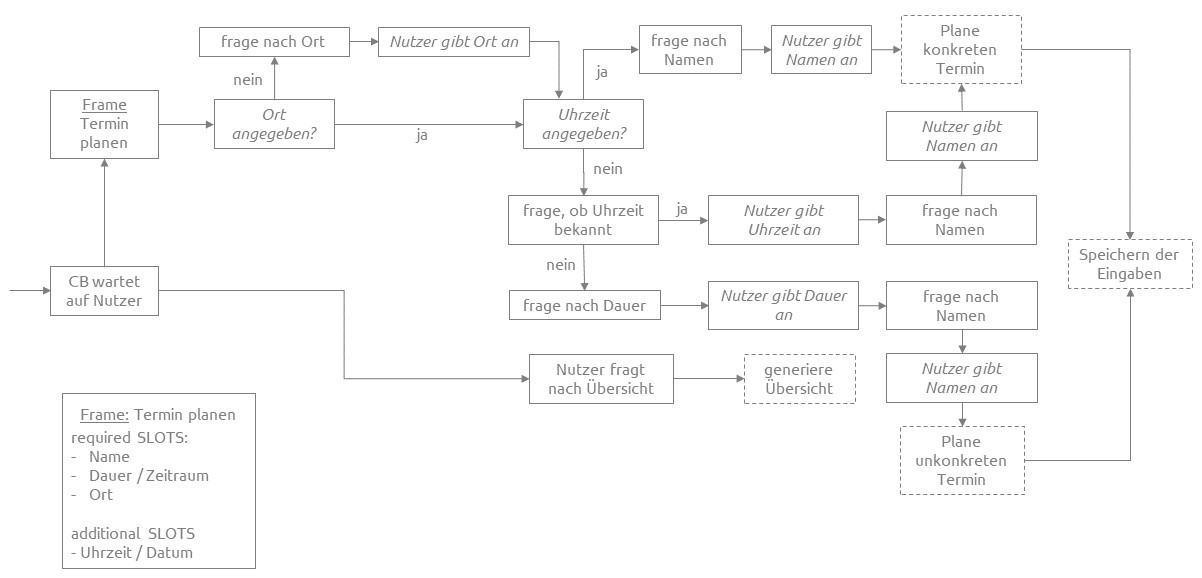
\includegraphics[width=\linewidth]{Dialogmodell_bild}\\
Der Nutzer kann einen Termin planen oder sich seinen derzeitigen Terminplan an Bild anzeigen lassen. Beim Planen von Terminen wird gefragt wo das Event stattfindet, welchen Namen das Event haben soll, ob es ein spezifisches (mit Start- und Endzeit) Event ist oder ein unspezifisches (nur Event-Dauer ist bekannt) und dann der Zeitrahmen/die Dauer.\\
Man kann auch bereits geplante Events wieder löschen. Dabei wählt der Nutzer mit Button, das er löschen will. 
Ein paar Small-Talk Optionen sind auch dabei, wie z.b fragen wie es dem Chatbot geht.\\\\
Der Bot ist eine Mischung aus Frame-basiert und Zustands-basiert. Das Planen von Event ist Frame-basiert, wo nach und nach die Fehlenden Slots (Ort, Event Name, spezifisches/unspezifisches Event,Dauer/Zeitrahmen) gefüllt werden. 
Während des Planens oder des Löschens eines Termins ist der Dialog eher System-Initiated, da die fehlenden Slots abgefragt werden, ansonsten User-Initiated.\\

\newpage
Beispiele:\\ 

\textbf{Plane ein Event mit bestimmtem Zeitrahmen}\\

\begin{framed}
\begin{tabular}{lr}
	\makecell[c]{JANUS} & \makecell[c]{USER} \\
 & plan an event at Rudower Chaussee 25 \\
Okay, what is the name of that event? & \\
 & Uni-Treffen\\
Do you know the exact time? & \\
 & Yes\\
Please tell me the time and date. & \\
 & Tomorrow from 4pm to 5pm\\
 \makecell[l]{Okay. Planned the event Uni-Treffen \\ at Rudower Chaussee 25, 12489 Berlin \\ from 14.08.2919 16:00 - 17:00.}
 \end{tabular}
\end{framed}

\hfill\\
\newpage
\textbf{Plane ein Event mit einer Event-Dauer}\\
\begin{framed}
\begin{tabular}{lr}
	\makecell[c]{JANUS} & \makecell[c]{USER} \\
	& schedule an event\\
	Where will this event take place? &\\
	& at Alten Försterei\\
	Okay, what is the name of that event? & \\
	& Fußball\\
	Do you know the exact time? & \\
	& nope\\
	Please tell me the duration of the event. & \\
	& 2 hours\\
	\makecell[l]{Okay. Planned the event Fußball \\ at Alte Försterei, 12555 Berlin \\ which will take 120min.}
\end{tabular}
\end{framed}
\hfill\\\\\\

\textbf{Erstellten Plan anzeigen lassen}\\
\begin{framed}
	\begin{tabular}{lr}
		\makecell[c]{JANUS} & \makecell[c]{USER} \\
		& please show me what has been scheduled.  \\
		That's what has been scheduled & \\
			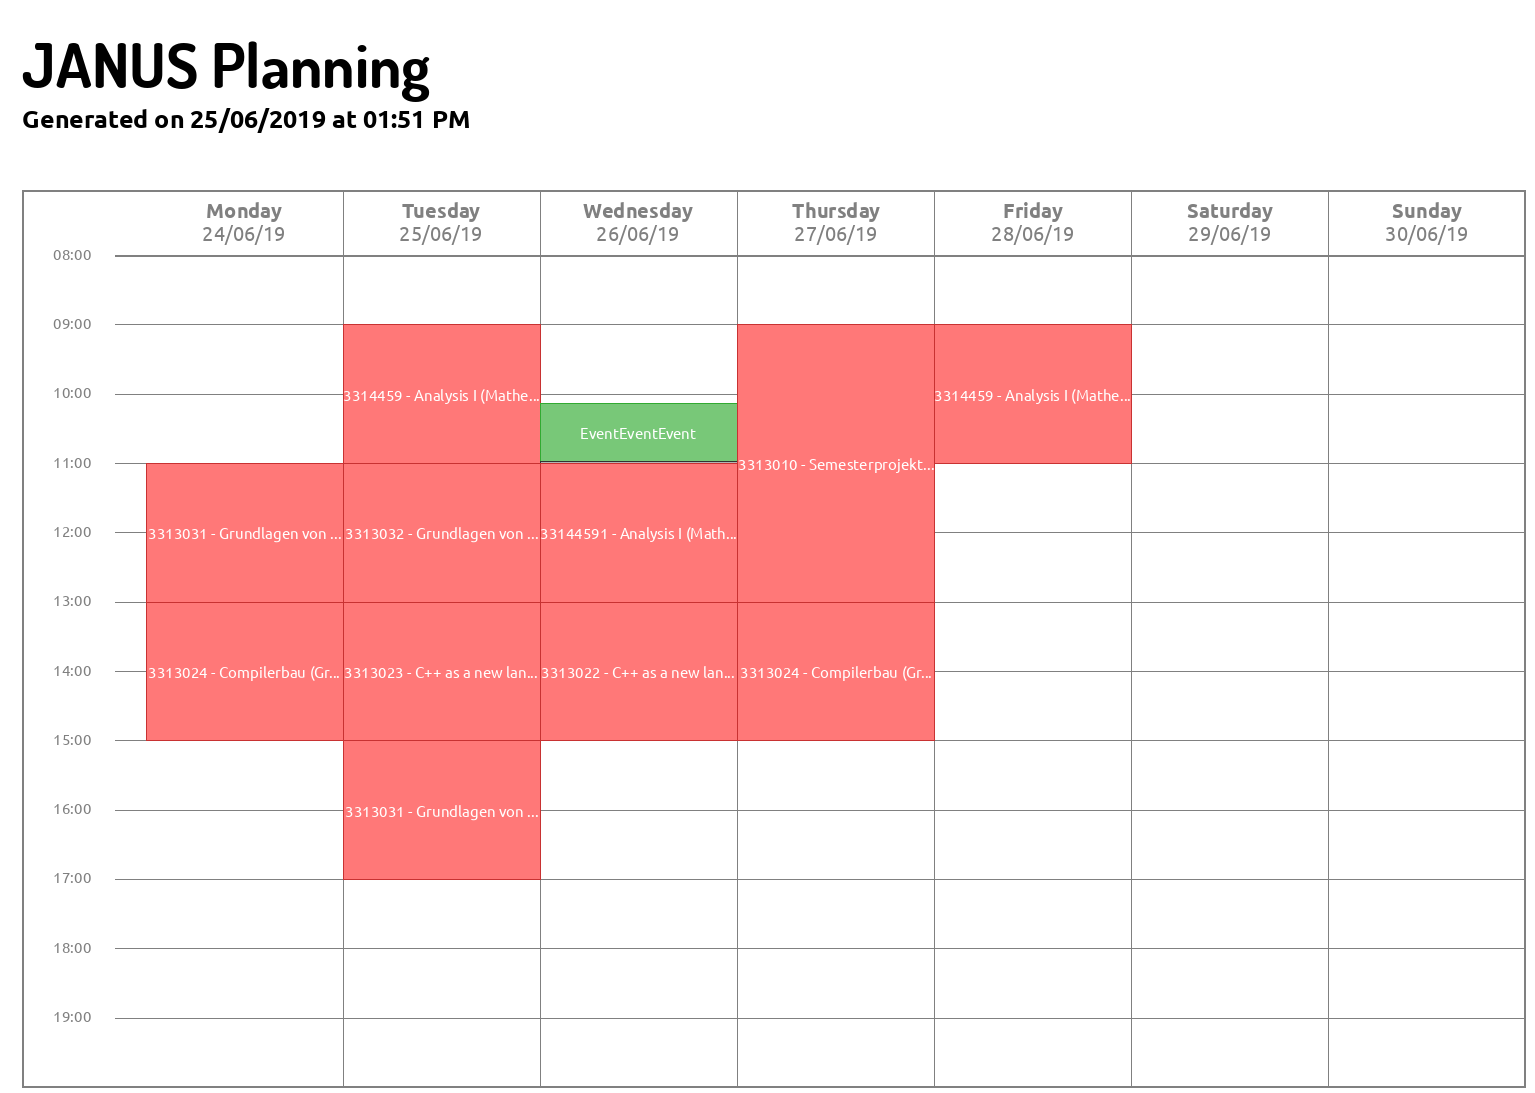
\includegraphics[width=0.30\linewidth]{show_plan} & 
	\end{tabular}
\end{framed}

\begin{framed}
	\begin{tabular}{lr}
		\makecell[c]{JANUS} & \makecell[c]{USER} \\
		& delete an event\\
		Which Event do you want to delete? &\\
			$\qquad$Uni-Treffen  & \\
			$\qquad$Fußball & \\
		& [wählt Fußball aus] \\
		Okay, deleted the event Fußball. & \\
	\end{tabular}
\end{framed}
\hfill\\
\end{document}
